\documentclass[dvipdfmx]{jsarticle}

\usepackage{ascmac}
\usepackage{url}
\usepackage[dvipdfmx]{hyperref}
\usepackage{pxjahyper}
\usepackage[dvipdfmx]{graphicx}
\usepackage{float}
\usepackage{listings,jlisting}

\hypersetup{
  colorlinks=true,
  urlcolor=cyan,
  linkcolor=black
}

\lstset{
  basicstyle={\ttfamily},
  identifierstyle={\small},
  commentstyle={\smallitshape},
  keywordstyle={\small\bfseries},
  ndkeywordstyle={\small},
  stringstyle={\small\ttfamily},
  frame={tb},
  breaklines=true,
  columns=[l]{fullflexible},
  numbers=left,
  xrightmargin=0zw,
  xleftmargin=3zw,
  numberstyle={\scriptsize},
  stepnumber=1,
  numbersep=1zw,
  lineskip=-0.5ex
}


\begin{document}

\section{実験目的・課題}

\begin{itemize}
  \item 単純な二次元データの分類
  \item 動物園の動物データ(多次元データ)の分類
  \item 食べ物の画像データの分類
\end{itemize}
を行う。

\section{実装方法}

\subsection{クラスタリングの手法について}

データのクラスタリングをする手法には以下のようなものがある。
\begin{itemize}
  \item 最短距離法
  \item 最長距離法
  \item 重心法
  \item 群平均法
  \item K-means法
\end{itemize}

最短距離法とは2つのクラスター同士について、
最も距離が小さいものから順にグループにしていくものである。
計算量が少ないが、ある1つのクラスタにひとつづつ吸収されてしまう
鎖効果が起こってしまうことがある。

最長距離法はクラスター間の距離をそのクラスター間の中で
最も遠いデータとし、その距離の小さいものから
クラスターにしていく手法である。
分類感度は高いがクラスター同士が離れてしまう拡散現象が起きることがある。

重心法はクラスターに属するデータの重心を決定し、
重心間の距離の小さい順にクラスターを
形成していく手法である。
計算量は多いが分類感度が良い。

群平均法は2つのクラスターに含まれるすべてのデータ間の距離
を計算し、その平均の値をクラスター間の距離として
クラスタリングをする手法である。
鎖効果や拡散現象をおこしにくい。

K-means法とはデータ数をn、クラスタ数をkとして、
以下のような手順で表されるアルゴリズムである。
\begin{enumerate}
  \item 各データ$d_i(i=1,\dots,n)$に対してランダムにクラスタを割り振る
  \item 各クラスタの中心$m_j(j=1,\dots,k)$を求める
  \item 各$d_i$と各$m_i$との距離を求め$d_i$を最も近いクラスタに割り当てなおす
  \item クラスタの割り当てが変化しなかった場合、終了する。\\そうでない場合手順2に戻る
\end{enumerate}
結果は、最初に割り振られたクラスタに依存し、
1回の結果で最良のものが得られるとは限らない。

\subsection{二次元データの分類}

\subsubsection{最短距離法}
二次元データ間の距離をユークリッド距離
$d = \sqrt{x^2 + y^2}$
で定義する。
これを最短距離法で分類することを考える。
最短距離法では単に短い距離のものから順にクラスタにまとめていけばよい。
これはクラスカル法で最小全域木を構築するのと
同様の手順で行うことができる。

クラスカル法とはグラフ理論において重み付き連結グラフの
最小全域木を求めることが出来る以下のようなアルゴリズムのことである。
\begin{enumerate}
  \item $cost(e_0) \leq cost(e_1) \leq \dots \leq cost(e_m)$が成り立つように辺を並び替える
  \item $T:=(V(G),\emptyset)$とする
  \item i=1..mについて、$E(T) \cup \{e_i\}$が閉路を含まないならば$E(T) := E(T) \cup \{e_i\}$とする
\end{enumerate}
二次元データを頂点、各点間の距離を重みとした辺からなるグラフを考える。
最初はN個の木(森)が存在し、このアルゴリズムが終了したときは1つの木だけが残っている。
この手順の途中で木の数がkになったときにアルゴリズムを終了すると、
k個のクラスタに分類することが出来ている。
クラスタの表現にはUnion Findというデータ構造を使用する。
これを実装したものをソースコード\ref{code:rust_emst}に示す。

\begin{lstlisting}[caption=Rustによる最短距離法の実装,label=code:rust_emst]
fn min_dist_method(data: &Vec<Point>, m: usize) -> Vec<usize> {
    let n = data.len();
    let mut edges: Vec<(f64, usize, usize)> = Vec::new();
    for i in 0..n {
        for j in i + 1..n {
            edges.push((calc_dist(data[i], data[j]), i, j));
        }
    }
    edges.sort_by(|a, b| a.partial_cmp(b).unwrap());
    let mut uni = Unionfind::new(n);
    for (_, i, j) in edges {
        if uni.tree_count == m {
            break;
        }
        uni.unite(i, j);
    }
    let mut cluster = (0..n).into_iter().map(|i| uni.root(i)).collect::<Vec<usize>>();
    cluster = compression(cluster);
    cluster
}
\end{lstlisting}

\subsubsection{群平均法}

群平均法ではクラスタ$c_a$と$c_b$の距離を
$c_a$の大きさ(所属しているデータの数)をN、$c_b$の大きさをMとして、
$\frac{1}{NM} \sum_{i=1}^{N} \sum_{j=1}^{M} d(c_{a_i},c_{b_j})$
として計算する。ここで、$d(p_i,p_j)$はデータ間の距離を計算する関数である。
こうして計算された距離の中で最小のものを併合していく。

クラスタはデータの追加が出来る集合とそれを管理する削除が出来る集合が必要であるため、
HashMapでVecを管理する。

\begin{lstlisting}[caption=群平均法の実装,label=code:rust_gam]
fn group_average_method(data: Vec<Point>, m: usize) -> HashMap<usize, Vec<Point>> {
    let mut cluster: HashMap<usize, Vec<Point>> = HashMap::new();
    let n = data.len();
    for i in 0..n {
        let vi = vec![data[i]];
        cluster.insert(i, vi);
    }
    let mut indexes = (0..n).into_iter().collect::<Vec<_>>();
    while cluster.len() > m {
        let (mut mi, mut mj) = (0, 0);
        let mut mdist = 1e10;
        for i in &indexes {
            for j in &indexes {
                if i < j {
                    let dist = calc_dist_average(&cluster[&i], &cluster[&j]);
                    if mdist > dist {
                        mdist = dist;
                        mi = *i;
                        mj = *j;
                    }
                }
            }
        }
        let mut clst_j = cluster.remove(&mj).unwrap();
        cluster.get_mut(&mi).unwrap().append(&mut clst_j);
        let rmidx = indexes.iter().position(|x| *x == mj).unwrap();
        indexes.remove(rmidx);
    }
    cluster
}
fn calc_dist_average(a: &Vec<Point>, b: &Vec<Point>) -> f64 {
    let mut sum_d: f64 = 0.;
    for ai in a {
        for bj in b {
            sum_d += calc_dist_point(*ai, *bj);
        }
    }
    sum_d / ((a.len() * b.len()) as f64)
}
\end{lstlisting}

\subsubsection{k-means法}

k-means法は初期状態によって結果が偏ってしまうことがあるので
複数回実行して分散の値が小さいものを結果が良かった
ものとして採択する。
分散の値は、各クラスタについて重心とのユークリッド距離で計算する。
重心の座標は次元ごとに平均をとったものとする。
その座標との距離の平均を$d_{mean}$とし、
各クラスタについて
$\sum_{i=1}^{N} (d(center,p_i)-d_{mean})^2$
を計算し、その値の平均値を分散とした。

\begin{lstlisting}[caption=k-means法の実装,label=code:kmeans]
fn k_means(data: &Vec<Point>, m: usize) -> (Vec<Vec<Point>>, Vec<usize>) {
    let n = data.len();
    let mut rng = rand::thread_rng();
    let mut cluster = (0..n).into_iter().map(|_| rng.gen_range(0..m)).collect::<Vec<_>>();
    let mut center = calc_center(&data, &cluster, m);
    loop {
        let mut new_cluser = vec![0; n];
        for i in 0..n {
            let mut d_min = 1e10;
            for j in 0..m {
                let d_cur = calc_dist(data[i], center[j]);
                new_cluser[i] = if d_min > d_cur {
                    d_min = d_cur;
                    j
                } else {
                    new_cluser[i]
                };
            }
        }
        if cluster == new_cluser {
            break;
        }
        cluster = new_cluser;
        center = calc_center(&data, &cluster, m);
    }
    let mut cluster_set: Vec<Vec<Point>> = vec![Vec::new(); m];
    for i in 0..n {
        cluster_set[cluster[i]].push(data[i]);
    }
    (cluster_set, cluster)
}
\end{lstlisting}


\subsection{多次元データの分類}

二次元データの分類の時と同様にクラスカル法を実行することで
最短距離法での分類を行う。
このときn次元データaとbの間の距離は
$\displaystyle d_{ab} = \sqrt{ \sum_{i=1}^{n}w_i(a_i - b_i)^2 }$
として計算した。ここで$w_i$は各系列に対する重みである。
ここで重みはランダムに決定し何度か実行し、
正解との差が小さいものを探した。


\subsection{画像データの分類}

画像データを次元の小さい多次元データに圧縮することで、
前節と同様に分類をすることができるようになる。

画像のデータはPythonのOpenCVではRGBを表す3要素からなる
配列の二次元配列である。
このRGBの値は$256^3=16777216$通り存在する。
各色についてその色が画像にいくつ含まれているかを
カウントした16777216次元データを比べることで画像間の
距離とすることでクラスタリングに必要な情報が得られる。
しかし、16777216個のデータを比較するのはデータの量が多すぎるため
困難である。
ここで、各画素の値を64で割り、0から255の値を0から3までの値に変換する。
こうすることで各画素を$4^3=64$通りの色に圧縮することが出来る。

画像を64次元データに圧縮することができたので最短距離法によって
画像の分類を実行する。

画像の分類結果を確認するために、Pythonのsubprocessパッケージ
のrun関数を使い、分類のたびに新たにディレクトリを作成し、
そこへ元画像のファイルをコピーした。

\section{結果と考察}

\subsection{二次元データの分類}

最短距離法、群平均法、k-means法のそれぞれでクラスタ4つ、
分散200のデータセットをクラスタリングした結果を
図\ref{fig:mdm_m4sd200}、\ref{fig:gam_m4sd200}、\ref{fig:km_m4sd200}に示す。

\begin{figure}[htbp]
  \begin{minipage}{0.5\hsize}
    \begin{center}
      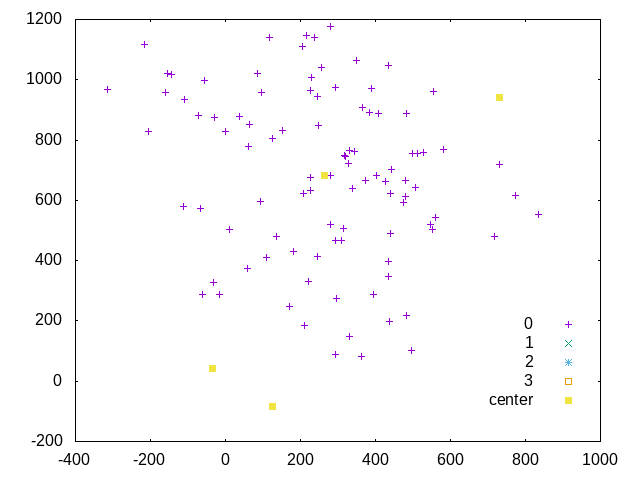
\includegraphics[width=1.0\hsize]{./pic/mdm/m4sd200_plot.png}
    \end{center}
    \caption{最短距離法によるクラスタリング}
    \label{fig:mdm_m4sd200}
  \end{minipage}
  \begin{minipage}{0.5\hsize}
    \begin{center}
      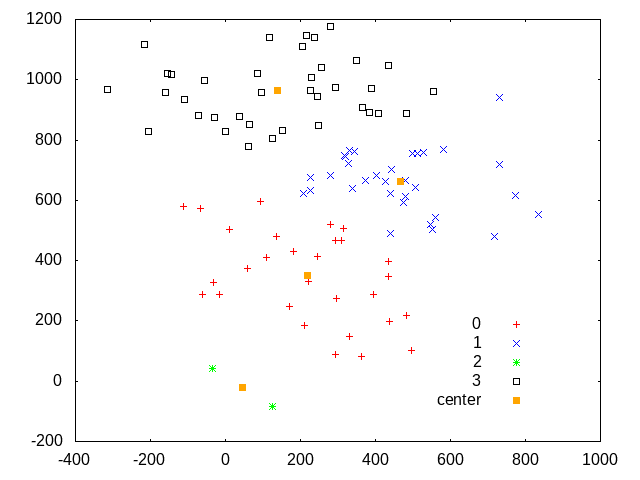
\includegraphics[width=1.0\hsize]{./pic/gam/m4sd200_plot.png}
    \end{center}
    \caption{群平均法によるクラスタリング}
    \label{fig:gam_m4sd200}
  \end{minipage}
\end{figure}
\begin{figure}[htbp]
  \centering
  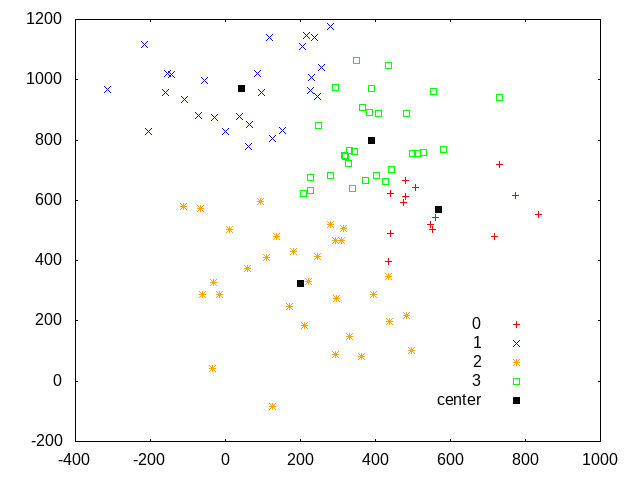
\includegraphics[width=0.5\hsize]{./pic/k_means/m4sd200_plot.png}
  \caption{k-means法によるクラスタリング}
  \label{fig:km_m4sd200}
\end{figure}


最短距離法によるクラスタリングでは、クラスタ1,2,3が1つの点からなる
クラスタになってしまっている。
これは、鎖効果が起こってしまったっためだと考えられる。
群平均法ではこれが改善され、k-means法ではさらに改善されて均等な
4つのクラスタに分類できていることがわかる。

最短距離法によるクラスタリングは図\ref{fig:mdm_m4sd200}のように
鎖効果が起こってしまうデメリットがあるが
最小全域木を構築する問題に帰着でき、
N個の点が与えられるとき
$O(Nlog(N))$と非常に高速に解くことが出来る。
具体的にはドロネーの三角形分割によって生成される
$O(N)$個の辺のみで最小全域木を構成することが出来る。


\subsection{多次元データの分類}

最短距離法によって分類した結果、以下のようになった。
正しい解との差は、2つだった。

\begin{verbatim}
  cluster 0:
  bass, carp, catfish, chub, dogfish, haddock, herring, pike, piranha, seahorse, sole, stingray, tuna
  cluster 1:
  aardvark, antelope, bear, boar, buffalo, calf, cavy, cheetah, deer, dolphin, elephant, fruitbat, giraffe, girl, goat, gorilla, hamster, hare, leopard, lion, lynx, mink, mole, mongoose, opossum, oryx, platypus, polecat, pony, porpoise, puma, pussycat, raccoon, reindeer, seal, sealion, squirrel, vampire, vole, wallaby, wolf
  cluster 2:
  chicken, crow, dove, duck, flamingo, gull, hawk, kiwi, lark, ostrich, parakeet, penguin, pheasant, rhea, skimmer, skua, sparrow, swan, vulture, wren
  cluster 3:
  clam, crab, crayfish, flea, gnat, honeybee, housefly, ladybird, lobster, moth, octopus, seawasp, slug, starfish, termite, wasp, worm
  cluster 4:
  frog, frog, newt, pitviper, slowworm, toad, tortoise, tuatara
  cluster 5:
  scorpion
  cluster 6:
  seasnake
\end{verbatim}

\subsection{画像データの分類}

画像の分類の結果は、
\begin{figure}[htbp]
  \begin{minipage}{0.5\hsize}
    \begin{center}
      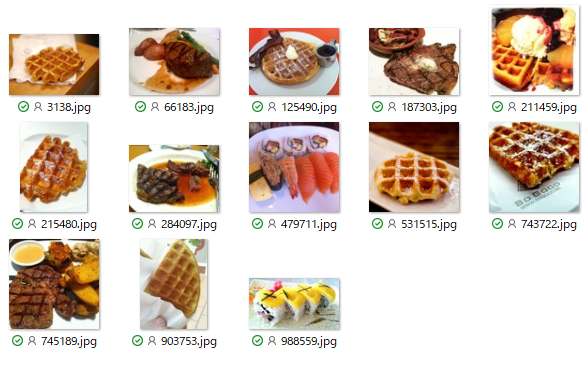
\includegraphics[width=1.0\hsize]{./pic/ic1.png}
    \end{center}
    \caption{クラスタ1}
    \label{fig:ic1}
  \end{minipage}
  \begin{minipage}{0.5\hsize}
    \begin{center}
      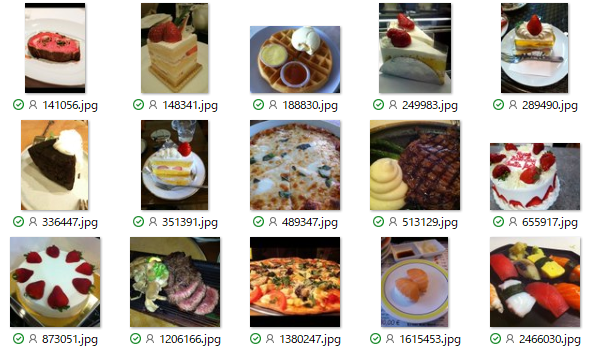
\includegraphics[width=1.0\hsize]{./pic/ic2.png}
    \end{center}
    \caption{クラスタ2}
    \label{fig:ic2}
  \end{minipage}
\end{figure}
\begin{figure}[htbp]
  \begin{minipage}{0.5\hsize}
    \begin{center}
      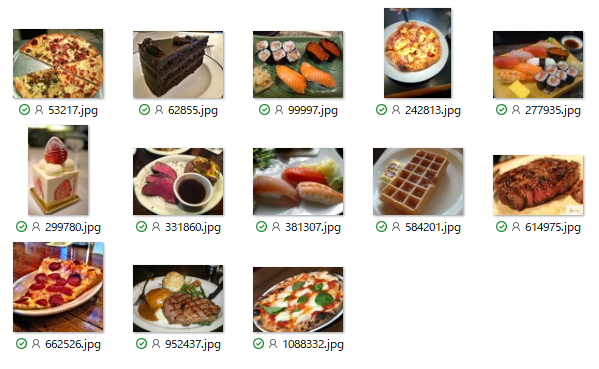
\includegraphics[width=1.0\hsize]{./pic/ic3.png}
    \end{center}
    \caption{クラスタ3}
    \label{fig:ic3}
  \end{minipage}
  \begin{minipage}{0.5\hsize}
    \begin{center}
      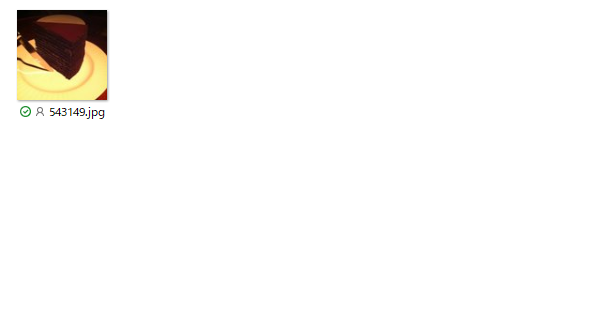
\includegraphics[width=1.0\hsize]{./pic/ic4.png}
    \end{center}
    \caption{クラスタ4}
    \label{fig:ic4}
  \end{minipage}
\end{figure}
\begin{figure}[htbp]
  \centering
  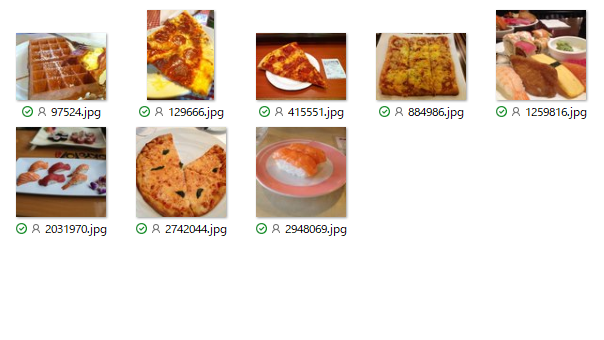
\includegraphics[width=0.7\hsize]{./pic/ic5.png}
  \caption{クラスタ5}
  \label{fig:ic5}
\end{figure}

\section{まとめ}

\newpage
\begin{thebibliography}{10}
  \bibitem{1} クラスター分析の手法2(階層クラスター分析)

  \url{https://www.albert2005.co.jp/knowledge/data_mining/cluster/hierarchical_clustering}

  \bibitem{2} k-means法を理解する

  \url{https://qiita.com/g-k/items/0d5d22a12a4507ecbf11}
\end{thebibliography}
\end{document}